\chapter{Auditing the Mint Application}
\label{mint:auditing}

In this chapter we discuss auditing and how the audit trail can be used for discovery.

As described in section \ref{aeolus:logging}, every security-related event is logged automatically by Aeolus. In addition, applications can log events of their own. We take advantage of this in the Mint system by logging application-specific events; an example is given in section \ref{audit:mint-example}.

Events are stored in a table that we will refer to as the \emph{LOG}. The LOG is useful for discovery, which can be done by means of a query over the table. Table \ref{table:bob-declass} and figure \ref{fig:user-activity} show two examples.

\begin{table}[h]
\begin{verbatim}
 secrecy | integrity | user  |  op_name   |        timestamp        
---------+-----------+-------+------------+-------------------------
 {11}    | {}        | Alex  | DECLASSIFY | 2012-06-13 21:57:06.876
 {11}    | {}        | Aline | DECLASSIFY | 2012-06-13 21:57:04.852
 {11}    | {}        | Jack  | DECLASSIFY | 2012-06-13 21:56:45.73
 {11}    | {}        | Jack  | DECLASSIFY | 2012-06-13 21:56:42.691
 {11}    | {}        | Mike  | DECLASSIFY | 2012-06-13 21:56:40.649
 {11}    | {}        | Mark  | DECLASSIFY | 2012-06-13 21:56:39.624
\end{verbatim}
\caption[Bob's Information Leaks]{Bob's Information Leaks. This table shows the declassifies of Bob's data tag from users other than Bob himself. The columns are as described in section \ref{sec:aeolus-event-attributes}.}
\label{table:bob-declass}
\end{table}

Table \ref{table:bob-declass} shows principals that declassified Bob's tag; thus, it shows which users accessed Bob's information. In a secure implementation of the Mint application, no user principal other than Bob's principal should be able to declassify Bob's tag. However we introduced a bug in our implementation of the Mint application to demonstrate how the LOG can be used for discovery, and hence we can see that many user principals were able to declassify Bob's tag - something that should never happen. In this example, the LOG helps us discover the leakage of Bob's information due to an application error.

\begin{figure}
\centering
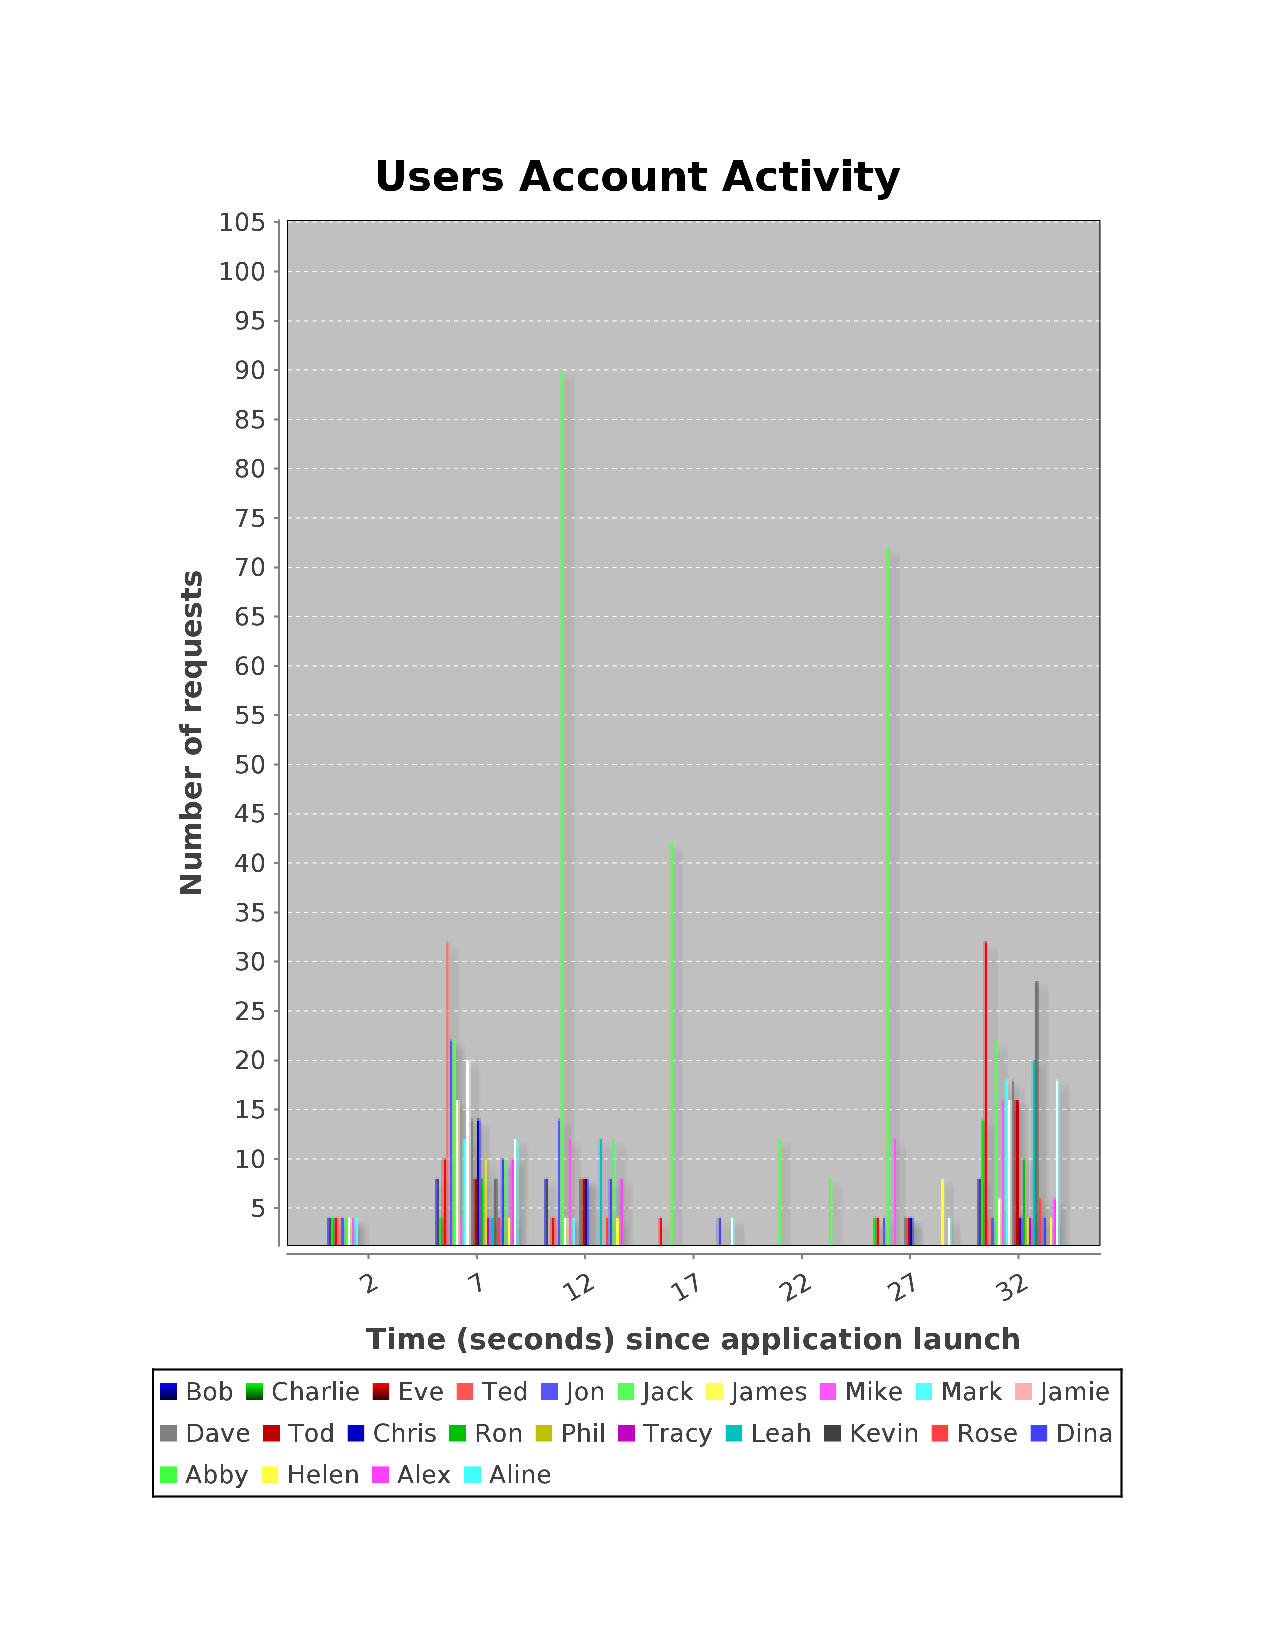
\includegraphics[width=\textwidth,height=\textheight,keepaspectratio]{figures/activity}
\caption[Mint User Activity Trend]{This graph shows the activity trend of each user. Notice that the activity for Jack spikes in the graph at multiple places. This could be the result of an attacker accessing his account and issuing requests to quickly retrieve all of Jack's financial information.}
\label{fig:user-activity}
\end{figure}

Figure \ref{fig:user-activity} shows a graph of how many user requests, for each user, caused a declassification of a user data tag for every 5-second period since the application launched; in other words, it shows the activity trend of each user. Any spike in the graph for a particular user means that that user was abnormaly active in certain periods of time. In this example, the LOG helps us discover if any user accounts have been compromised.

In the following section we describe how the data for Figure \ref{fig:user-activity} can be extracted from the LOG.

\section{Detecting Suspicious User Activity}
\label{audit:mint-example}
In order to gather the information necessary to produce the graph in figure \ref{fig:user-activity}, we add application-specific events to the LOG for each different action the user takes.

For example, when Bob signs up successfully with our application, we record his username, ``Bob'', as well as his data tag and the principal authoritative for that tag. This is done using the following call\footnote{Recording the principal ID and the number of the tag is enough to retrieve the full information about a principal and a tag from the AS.}:

\begin{lstlisting}[language=Java, label=code:create-event]
  AeolusLib.createEvent(``mint-user-signup'', 
    Arrays.asList(
      new String[] {``Bob'', ``5'', ``10''}));
\end{lstlisting}

\noindent
This call causes a \emph{sign up} event to be added to the LOG. To obtain a table detailing the username, principal, data tag and other sign-up information of all users, we use the following SQL query based on our application-specific events\footnote{\emph{to\_array} is a procedure that turns a comma-delimited string into a PSQL array.}:

\begin{lstlisting}[language=SQL, deletendkeywords={TIMESTAMP}, label=code:mint-signup]
select to_array(app_arg)[0] as pid, 
  to_array(app_arg)[1] as username, 
  to_array(app_arg)[2] as tag, 
  timestamp as signed_up, 
  event_counter 
from events 
where op_name='mint-user-signup'
\end{lstlisting}

\noindent
Table \ref{table:users-info} shows a possible result of running the query, with some extra information about the time when each user signed up.

\begin{table}
\begin{verbatim}
 pid | username | substring |        signed_up        | e_ctr 
-----+----------+-----------+-------------------------+------
   6 | wissam   | 4         | 2012-06-13 21:56:36.207 |  131
   9 | david    | 7         | 2012-06-13 21:56:36.207 |  445
  12 | dan      | 10        | 2012-06-13 21:56:37.338 |  793
  13 | Bob      | 11        | 2012-06-13 21:56:37.338 | 1148
  14 | Charlie  | 12        | 2012-06-13 21:56:37.338 | 1211
  15 | Eve      | 13        | 2012-06-13 21:56:37.338 | 1274
  16 | Ted      | 14        | 2012-06-13 21:56:37.338 | 1337
  17 | Jon      | 15        | 2012-06-13 21:56:37.338 | 1400
  18 | Jack     | 16        | 2012-06-13 21:56:37.338 | 1463
  19 | James    | 17        | 2012-06-13 21:56:37.338 | 1526
  20 | Mike     | 18        | 2012-06-13 21:56:37.338 | 1589
  21 | Mark     | 19        | 2012-06-13 21:56:37.338 | 1652
  22 | Jamie    | 20        | 2012-06-13 21:56:38.578 | 1715
  23 | Dave     | 21        | 2012-06-13 21:56:38.578 | 1778
  24 | Tod      | 22        | 2012-06-13 21:56:38.578 | 1841
  25 | Chris    | 23        | 2012-06-13 21:56:38.578 | 1904
  26 | Ron      | 24        | 2012-06-13 21:56:38.578 | 1967
  27 | Phil     | 25        | 2012-06-13 21:56:38.578 | 2030
  28 | Tracy    | 26        | 2012-06-13 21:56:38.578 | 2093
  29 | Leah     | 27        | 2012-06-13 21:56:38.578 | 2156
  30 | Kevin    | 28        | 2012-06-13 21:56:38.578 | 2219
  31 | Rose     | 29        | 2012-06-13 21:56:38.578 | 2282
  32 | Dina     | 30        | 2012-06-13 21:56:38.578 | 2345
  33 | Abby     | 31        | 2012-06-13 21:56:38.578 | 2408
  34 | Helen    | 32        | 2012-06-13 21:56:38.578 | 2471
  35 | Alex     | 33        | 2012-06-13 21:56:38.578 | 2534
  36 | Aline    | 34        | 2012-06-13 21:56:38.578 | 2597
\end{verbatim}
\caption[Mint Users Information]{Mint Users Information. This is a table detailing the information about users signing up during a simulated run of the Mint application. The \emph{pid} column denotes the user's principal, the \emph{username} column denotes the user's username, the \emph{tag} column denotes the user's data tag, the \emph{signed\_up} column denotes the time at which the sign up event took place, and the \emph{e\_ctr} column denotes the unique event\_counter number of the sign up event.}
\label{table:users-info}
\end{table}

Finally, we can obtain the information necessary to create the graph in figure \ref{fig:user-activity} using the following query:

\begin{lstlisting}[language=SQL, deletendkeywords={TIMESTAMP}, label=code:query-accesses]
select e.count, users.username, 
  e.to_timestamp as timestamp 
from (select count(*), tags_modified, 
  (to_timestamp(((extract(epoch 
    from events.timestamp)/5)::int)*5)) 
  from events where tags_modified 
  in (select tag from users) group by
  (to_timestamp(((extract (epoch 
    from events.timestamp)/5)::int)*5)), 
  tags_modified) 
as e inner join users on e.tags_modified=users.tag
\end{lstlisting}

Table \ref{table:jack-activity} shows a the result of a modified version of this query that shows information just for the user Jack. This query provides us with a count of how many requests by Jack caused a declassification of a user data tag for every 5-second period of time since the application launch.

\begin{table}
\begin{quote}
\begin{verbatim}
 count | username |       timestamp        
-------+----------+------------------------
    22 | Jack     | 2012-06-13 21:56:40-04
     4 | Jack     | 2012-06-13 21:56:35-04
    42 | Jack     | 2012-06-13 21:56:50-04
    72 | Jack     | 2012-06-13 21:57:00-04
    90 | Jack     | 2012-06-13 21:56:45-04
    12 | Jack     | 2012-06-13 21:56:55-04
    22 | Jack     | 2012-06-13 21:57:05-04
\end{verbatim}
\end{quote}
\caption[Mint Account activity for user Jack]{Mint Account activity for user Jack. This table shows the number of declassifies done by Jack's principal in each five-second period since the application launched. The \emph{count} denotes such number. The \emph{username} column denotes the user who's data tag is in question. The \emph{timestamp} column denotes the start of the 5-second period. A table containing similar information for all users would be a precursor to producing the graph in figure \ref{fig:user-activity}, but here we only show this data for user Jack for simplicity.}
\label{table:jack-activity}
\end{table}
